% TeX_Agent 代码文档
% 编译建议：xelatex main.tex（需 ctex 宏包）
\documentclass[12pt,a4paper]{ctexart}

\usepackage{geometry}
\geometry{margin=2.5cm}
\usepackage{graphicx}
\usepackage{hyperref}
\usepackage{array}
\usepackage{seqsplit}
\usepackage{booktabs}
\usepackage{longtable}
\usepackage{enumitem}
\usepackage{xcolor}
\usepackage{listings}

\hypersetup{
    colorlinks=true,
    linkcolor=blue,
    urlcolor=blue,
    citecolor=blue
}

\lstset{
    basicstyle=\ttfamily\small,
    breaklines=true,
    frame=single,
    backgroundcolor=\color{gray!8}
}

\newcommand{\toolfile}[1]{{\ttfamily\seqsplit{#1}}}

\title{Tex\_Agent 软件 SBOM 与代码说明文档}
\author{团队成员：毛伟翔、于天泽、乔雨霖、唐俊涛}
\date{\today}

\begin{document}
\maketitle
\begingroup
\hypersetup{linkcolor=black}
\tableofcontents
\endgroup
\newpage

\section{代码结构与模块依赖}

本节给出 TeX\_Agent 主要目录的\textbf{浅层结构树}与\textbf{模块依赖关系}，
层级深度控制在 1--2 级，便于从整体上把握系统构成（详细文件说明见后续各章）。

\subsection{主要目录结构}

\begin{lstlisting}[language={},basicstyle=\ttfamily\footnotesize]
TeX_Agent/
|-- main.py / check.py / check_text.py / overleaf.py   # 程序入口
|-- start_all.bat            # Windows 一键启动 Chat + Writing 双服务
|-- config/                  # 统一配置与工作流注册表
|-- core/                    # 消息协议、状态、CLI 编排核心
|-- workflow/                # LangGraph 工作流引擎
|-- agents/                  # 多智能体实现
|-- tools/                   # 可插拔工具层
|-- context/ + memory/ + rag/   # 上下文 / 记忆 / 检索增强
|-- router/                  # Plan 模式任务规划
|-- latex/                   # LaTeX 诊断修复子系统
|-- ui/                      # Web UI / Overleaf 编辑器 / Ghost 窗口
|-- cli/ + utils/            # 终端命令框架 / 通用工具
|-- scripts/                 # 启动脚本
`-- tests/ + test/           # 测试代码（详见测试文档）
\end{lstlisting}

\subsection{测试说明}

项目提交了额外的测试文档，用例范围、目录组织、执行方式与结果等详情请参阅测试文档，本文档不再展开各测试文件说明。

测试代码主要位于仓库根目录 \texttt{tests/}；运行配置见 \texttt{pytest.ini}。

\subsection{模块依赖关系图}

下图展示各主要文件夹之间的\textbf{调用/依赖方向}（箭头表示「依赖或被调用」关系，非文件包含关系）。

\begin{center}
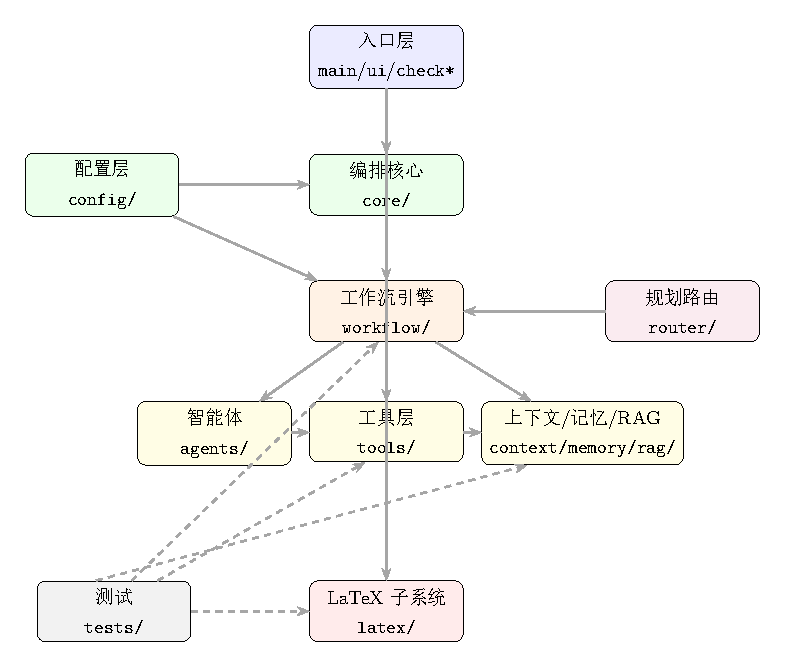
\includegraphics[width=\textwidth]{module_dependency_diagram.pdf}
\end{center}

\noindent\textbf{读图说明：}
\begin{itemize}[leftmargin=2em]
    \item \textbf{入口层}（\texttt{main.py}、\texttt{ui/}、\texttt{check*.py}）统一委托 \texttt{core/agent\_cli.py} 编排执行。
    \item \textbf{config/} 为全局配置源，被 \texttt{core/}、\texttt{workflow/}、\texttt{agents/} 等读取。
    \item \textbf{workflow/} 是执行中枢，调度 \texttt{agents/}、\texttt{tools/}，并借助 \texttt{context/}、\texttt{memory/}、\texttt{rag/} 拼装 Prompt。
    \item \textbf{router/} 仅在 Plan 模式下介入，将用户任务分解为动态图后交给 \texttt{workflow/}。
    \item \textbf{latex/} 作为独立子系统，主要由 \texttt{tools/latex\_*} 与 \texttt{ui/ghost/} 调用。
    \item 虚线表示 \texttt{tests/} 对各个功能模块的验证依赖（测试调用，非运行时依赖）。
\end{itemize}

\subsection{主要目录作用速查}

\begin{longtable}{@{}p{0.22\textwidth}p{0.36\textwidth}p{0.30\textwidth}@{}}
\toprule
\textbf{目录} & \textbf{作用} & \textbf{主要依赖} \\
\midrule
\endhead
\texttt{config/} & 环境变量、工作流 JSON、上下文 Profile、Planner Schema & 无（被各层读取） \\
\texttt{core/} & 消息协议、WorkflowState、TeXAgentCLI 编排入口 & \texttt{config/}, \texttt{workflow/} \\
\texttt{workflow/} & JSON/TaskPlan $\rightarrow$ LangGraph 图编译与执行 & \texttt{config/}, \texttt{agents/}, \texttt{tools/} \\
\texttt{agents/} & LLM 智能体（Simple/Multi/Reflection 等） & \texttt{core/}, \texttt{tools/} \\
\texttt{tools/} & 可插拔工具（arXiv、PDF、LaTeX、RAG 等） & \texttt{latex/}, \texttt{rag/}, \texttt{memory/} \\
\texttt{context/} & GSSC 上下文流水线，拼装 Agent Prompt & \texttt{config/}, \texttt{memory/} \\
\texttt{memory/} & 分支记忆、用户画像持久化 & \texttt{core/} \\
\texttt{rag/} & ChromaDB 向量检索管道 & \texttt{config/} \\
\texttt{router/} & Plan 模式 MAS 任务分解与图生成 & \texttt{config/}, \texttt{workflow/} \\
\texttt{latex/} & LaTeX 项目索引、L1/L2/L3 诊断修复、Ghost 窗口 & 系统 TeX 工具链（chktex/latexmk） \\
\texttt{ui/} & Web 聊天 UI、Overleaf 编辑器、Ghost 浮层 & \texttt{core/}, \texttt{latex/}, \texttt{rag/} \\
\texttt{cli/} & 终端 REPL 命令注册与分支管理 & \texttt{core/} \\
\texttt{utils/} & 日志、并发、回复格式化、取消控制等 & \texttt{config/} \\
\texttt{tests/}、\texttt{test/} & pytest 测试与演示脚本；详见测试文档 & 被测模块 \\
\bottomrule
\end{longtable}

\section{软件 SBOM 清单}

本节按软件物料清单（SBOM）要求，说明各模块的\textbf{来源分类}、\textbf{大模型 Prompt 溯源}、
\textbf{人工加工说明}及\textbf{第三方开源依赖}。

\subsection{来源分类说明}

本项目代码来源分为四类：

\begin{description}[leftmargin=4em,style=nextline]
    \item[自研]
    项目组成员在仓库中独立设计并实现的功能代码。

    \item[大模型生成]
    依据 \texttt{doc/} 目录下 Prompt 文档及其他辅助说明性文字，由大语言模型生成的\textbf{初始项目骨架}与接口占位代码。

    \item[大模型辅助生成]
    在大模型建议或草稿基础上，由成员审核、测试、修改后纳入仓库的代码。

    \item[复用开源]
    通过 \texttt{requirements.txt} 引入的第三方 Python 库，或前端 vendor 目录中的开源 JS 库。
\end{description}

\subsection{大模型生成内容与 Prompt 溯源}

\begin{longtable}{@{}>{\raggedright\arraybackslash}p{0.20\textwidth}>{\raggedright\arraybackslash}p{0.34\textwidth}>{\raggedright\arraybackslash}p{0.36\textwidth}@{}}
\toprule
\textbf{生成内容} & \textbf{Prompt / 设计文档} & \textbf{说明} \\
\midrule
\endhead
系统总体目录结构与初始框架骨架 &
\texttt{doc/代码框架要求.md} &
要求大模型输出目录树、README、可运行 MVP 及标注 \texttt{[扩展]} 的接口占位。
关联背景：\texttt{doc/论文写作协作智能体开发项目计划.md}。 \\

多智能体工作流基础图结构 &
\texttt{doc/代码框架要求.md}（第一节 LangGraph Workflow） &
含 Design$\rightarrow$Think$\rightarrow$Execute 链式节点、\texttt{WorkflowState}、节点包装器。 \\

Agent / Tool / Memory / Router 抽象基类 &
\texttt{doc/代码框架要求.md}（第二至六节） &
\texttt{ReActAgent}、\texttt{PlanAndSolveAgent}、\texttt{BaseRouter} 等
\texttt{[扩展]} 占位接口。 \\

\texttt{tests/} 单元测试文件 &
无独立 Prompt 存档（大模型辅助生成） &
测试骨架由大模型辅助产出，成员后续补充用例、修正断言并用于回归验证。 \\

LaTeX 子系统设计方案（非直接代码生成） &
\texttt{doc/TeX\_Agent 核心系统设计方案：}\newline
\texttt{LaTeX 结构理解与智能诊断体系.md} &
作为 \texttt{latex/} 子系统的设计依据；具体实现为成员自研。 \\

Task/Plan Prompt 注入机制说明 &
\texttt{doc/prompt\_injection\_map\_}\newline\texttt{task\_plan.md} &
记录 \texttt{task} 与 \texttt{plan} 链路中 Prompt 拼接与注入位置（审计文档，非代码生成 Prompt）。 \\
\bottomrule
\end{longtable}

\subsection{人工加工与演进说明}

大模型仅提供\textbf{可运行的最小骨架}与\textbf{扩展接口占位}；项目的实际业务能力均由小组成员在此基础上人工开发完成（部分有大模型辅助，但后续提交的代码都经过开发人员人工审核和测试）：

\begin{enumerate}[leftmargin=2em]
    \item \textbf{框架填充与扩展}：大模型最初生成的代码框架仅作示意，方便成员预先了解可能的接口，便于并行开发，后续开发过程中开发者会根据实际情况修改和扩展最初的框架（并同步给其他开发者）。在 \texttt{SimpleAgent}、\texttt{workflow/nodes.py}、\texttt{graph\_builder.py} 等大模型骨架上，实现了条件边、并行分叉/汇聚、Web 自定义工作流、Plan 模式动态构图等完整框架能力。
    \item \textbf{业务功能自研}：LaTeX 诊断修复流水线、论文 checklist 审查、Ghost 幽灵窗口、Overleaf 编辑器、latex 论文写作、RAG 集成、Web 辅助工具等均为按需求独立开发。
    \item \textbf{测试与纠错}：\texttt{tests/} 中大模型辅助生成的测试文件，经成员人工审阅后用于\textbf{功能验证与辅助纠错}，并非直接可交付的运行时代码。
    \item \textbf{大模型辅助}：团队开发中仍会使用大模型进行辅助开发或辅助编写代码，但大模型生成的代码均会被人工第一时间审核和测试，确保代码质量和功能正确性。
\end{enumerate}

\subsection{按目录来源标注总表}

\begin{longtable}{@{}>{\raggedright\arraybackslash}p{0.21\textwidth}>{\raggedright\arraybackslash}p{0.12\textwidth}>{\raggedright\arraybackslash}p{0.25\textwidth}>{\raggedright\arraybackslash}p{0.31\textwidth}@{}}
\toprule
\textbf{目录/模块} & \textbf{来源} & \textbf{Prompt 溯源} & \textbf{人工加工要点} \\
\midrule
\endhead
\texttt{core/}（消息/状态/异常） & 大模型生成 + 自研 & \texttt{doc/代码框架要求.md} & 扩展 reducer、TeXAgentCLI 完整编排 \\
\texttt{agents/}（基类骨架） & 大模型生成 + 自研 & \texttt{doc/代码框架要求.md} & 实现 SimpleAgent、MultiSimpleAgent、ReflectionAgent \\
\texttt{workflow/}（基础图） & 大模型生成 + 自研 & \texttt{doc/代码框架要求.md} & 条件边、并行节点、registry、run\_dump \\
\texttt{memory/}（接口） & 大模型生成 + 自研 & \texttt{doc/代码框架要求.md} & BranchMemory、UserPersonaMemory 完整实现 \\
\texttt{router/} & 大模型生成 + 自研 & \texttt{doc/代码框架要求.md} & AutoAgentsMASPlanner 完整实现 \\
\texttt{context/} & 大模型辅助 + 自研 & — & GSSC 流水线、context\_profiles 集成 \\
\texttt{config/} & 大模型辅助 + 自研 & — & 上下文 Profile、25+ 工作流 JSON、Planner Schema \\
\texttt{tools/}（arxiv 骨架） & 大模型生成 + 自研 + 复用开源 & \texttt{doc/代码框架要求.md} & 30+ 业务工具（PDF、checklist、LaTeX 等） \\
\texttt{latex/} & 大模型辅助 + 自研 & 设计文档（见上表） & 完整诊断修复、Ghost、Watch 服务 \\
\texttt{rag/} & 大模型辅助 + 自研 + 复用开源 & — & ChromaDB 管道、CLI 工具 \\
\texttt{ui/} & 大模型辅助 + 自研 & — & Web UI、Overleaf、Ghost 前端 \\
\texttt{cli/}、\texttt{utils/} & 大模型辅助 + 自研 & — & 命令框架、日志、取消控制等 \\
\texttt{check.py}\newline\texttt{check\_text.py} & 自研 & — & 批量审查脚本 \\
\texttt{tests/} & 大模型辅助 + 自研 & — & 补充用例、集成测试、夹具维护 \\
\bottomrule
\end{longtable}

\subsection{第三方开源依赖清单}

以下依赖来自 \texttt{requirements.txt}，按功能分组列出（版本约束以文件为准）。

\subsubsection{工作流与 LLM 框架}

\begin{longtable}{@{}p{0.32\textwidth}p{0.14\textwidth}p{0.44\textwidth}@{}}
\toprule
\textbf{包名} & \textbf{最低版本} & \textbf{本项目用途} \\
\midrule
\endhead
\texttt{langgraph} & 0.2.0 & 多智能体工作流图编排引擎 \\
\texttt{langchain} & 0.3.0 & LLM 应用框架（辅助） \\
\texttt{langchain-openai} & 0.2.0 & OpenAI 兼容 API 接入 \\
\texttt{langchain-core} & 0.3.0 & LangChain 核心抽象 \\
\texttt{pydantic} & 2.0.0 & 数据模型校验（WorkflowMessage、LaTeX 模型等） \\
\texttt{python-dotenv} & 1.0.0 & \texttt{.env} 环境变量加载 \\
\texttt{google-genai} & 1.0.0 & Gemini 多模态 API \\
\texttt{httpx} & 0.27.0 & 异步 HTTP 客户端 \\
\texttt{arxiv} & 2.1.0 & arXiv 文献检索 API \\
\bottomrule
\end{longtable}

\subsubsection{Web 服务}

\begin{longtable}{@{}p{0.32\textwidth}p{0.14\textwidth}p{0.44\textwidth}@{}}
\toprule
\textbf{包名} & \textbf{最低版本} & \textbf{本项目用途} \\
\midrule
\endhead
\texttt{fastapi} & 0.110.0 & Web UI / Overleaf / Ghost HTTP 服务 \\
\texttt{uvicorn[standard]} & 0.27.0 & ASGI 服务器 \\
\texttt{anyio} & 4.0.0 & 异步 I/O 兼容层 \\
\texttt{python-multipart} & 0.0.9 & 文件上传解析 \\
\bottomrule
\end{longtable}

\subsubsection{RAG 与向量检索}

\begin{longtable}{@{}p{0.32\textwidth}p{0.14\textwidth}p{0.44\textwidth}@{}}
\toprule
\textbf{包名} & \textbf{最低版本} & \textbf{本项目用途} \\
\midrule
\endhead
\texttt{chromadb} & 0.5.0 & 本地向量数据库（RAG 持久化） \\
\bottomrule
\end{longtable}

\subsubsection{LaTeX 诊断}

\begin{longtable}{@{}p{0.32\textwidth}p{0.14\textwidth}p{0.44\textwidth}@{}}
\toprule
\textbf{包名} & \textbf{最低版本} & \textbf{本项目用途} \\
\midrule
\endhead
\texttt{pylatexenc} & 2.10 & LaTeX 源码解析辅助 \\
\texttt{watchdog} & 4.0.0 & 目录文件监视（Ghost / Watch 服务） \\
\multicolumn{3}{l}{\textit{系统级依赖（非 pip）：TeX Live / MiKTeX、latexmk、chktex}} \\
\bottomrule
\end{longtable}

\subsubsection{PDF 与文档解析}

\begin{longtable}{@{}p{0.32\textwidth}p{0.14\textwidth}p{0.44\textwidth}@{}}
\toprule
\textbf{包名} & \textbf{最低版本} & \textbf{本项目用途} \\
\midrule
\endhead
\texttt{pymupdf} & 1.24.0 & PDF 文本快速提取 \\
\texttt{pypdf} & 4.2.0 & PDF 读取 \\
\texttt{pdfplumber} & 0.11.0 & PDF 版面分析 \\
\texttt{PyPDF2} & 3.0.0 & PDF 读取（兼容） \\
\texttt{python-docx} & 1.1.0 & Word 文档读取 \\
\texttt{docling} & 2.0 & 文档结构化解析（PDF$\rightarrow$MD+JSON） \\
\bottomrule
\end{longtable}

\subsubsection{可视化、工具与测试}

\begin{longtable}{@{}p{0.32\textwidth}p{0.14\textwidth}p{0.44\textwidth}@{}}
\toprule
\textbf{包名} & \textbf{最低版本} & \textbf{本项目用途} \\
\midrule
\endhead
\texttt{matplotlib} & 3.8.0 & Web 工具箱图表绘制 \\
\texttt{qrcode[pil]} & 7.4.0 & 二维码生成 \\
\texttt{pytest} & 7.0.0 & 单元/集成测试框架 \\
\texttt{pytest-asyncio} & 0.21.0 & 异步测试支持 \\
\bottomrule
\end{longtable}

\subsubsection{前端 vendor 开源库（非 pip）}

\begin{longtable}{@{}>{\raggedright\arraybackslash}p{0.50\textwidth}@{\hspace{3mm}}>{\raggedright\arraybackslash}p{0.44\textwidth}@{}}
\toprule
\textbf{文件} & \textbf{用途} \\
\midrule
\endhead
\toolfile{ui/web/static/vendor/marked.min.js} & Markdown 渲染 \\
\toolfile{ui/web/static/vendor/purify.min.js} & HTML 消毒（XSS 防护） \\
\toolfile{ui/web/static/vendor/highlight.min.js} & 代码语法高亮 \\
\toolfile{ui/overleaf/static/vendor/pdf.min.js} & PDF.js 预览 \\
\bottomrule
\end{longtable}


\section{项目概述}

TeX\_Agent 是基于 \textbf{LangGraph + 多智能体（MAS）} 架构的学术论文写作智能辅助系统。
系统覆盖文献检索、LaTeX 结构诊断与修复、论文写作和润色、论文合规审查（checklist）、RAG 知识检索、多分支对话上下文管理、工作流可视化编排等功能。

\subsection{架构总览}

\begin{itemize}[leftmargin=2em]
    \item \textbf{入口层}：\texttt{start\_all.bat}（Windows 一键启动双 Web 服务）、\texttt{main.py}（CLI REPL）；\newline
          \texttt{ui/web/server.py}（Chat Mode）、\texttt{ui/overleaf/server.py}（Writing Mode）；\newline
          \texttt{check.py}、\texttt{check\_text.py}（批量审查脚本）
    \item \textbf{编排层}：\texttt{core/agent\_cli.py} 的 \texttt{TeXAgentCLI} 串联记忆、分支、工作流
    \item \textbf{工作流引擎}：\texttt{workflow/} 将 JSON/TaskPlan 编译为 LangGraph 图并执行节点
    \item \textbf{智能体层}：\texttt{agents/} 提供 \texttt{SimpleAgent}、\texttt{MultiSimpleAgent} 等
    \item \textbf{工具层}：\texttt{tools/} 可插拔工具（arXiv、PDF 解析、LaTeX 诊断、RAG 检索等）
    \item \textbf{LaTeX 子系统}：\texttt{latex/} 项目索引、诊断修复、润色建议、LaTeX 写作、文件监视与幽灵窗口
    \item \textbf{支撑模块}：\texttt{config/}、\texttt{context/}、\texttt{memory/}、\texttt{rag/}、\texttt{router/}
\end{itemize}

\subsection{快速启动}

环境配置完成后，Windows 下可\textbf{双击根目录 \texttt{start\_all.bat}} 一键启动两个 Web 服务
（与 \texttt{README.md} 快速启动说明一致）：

\begin{longtable}{@{}p{0.16\textwidth}p{0.30\textwidth}p{0.46\textwidth}@{}}
\toprule
\textbf{服务} & \textbf{地址} & \textbf{说明} \\
\midrule
\endhead
Chat Mode & \texttt{http://127.0.0.1:8765/} & Web UI：工作流编排、论文审查、RAG 等 \\
Writing Mode & \texttt{http://127.0.0.1:8772/} & Overleaf 风格在线 LaTeX 编辑器 \\
\bottomrule
\end{longtable}

\noindent 脚本会先清理 8765/8772 端口上的旧进程，再分别在独立控制台窗口启动
\texttt{python -m ui.web.server} 与 \texttt{python -m ui.overleaf.server}。
亦可手动分别执行上述命令；Linux/macOS 可参考 \texttt{scripts/start-texagent-web.sh} 启动 Chat Mode。

\subsection{文档范围说明}

本文档基于仓库源码写作（\url{https://github.com/BCyyyyyyTZ/Tex_Agent.git}），\textbf{排除}以下内容：
\begin{itemize}[leftmargin=2em]
    \item \texttt{.gitignore} 中忽略的路径（如 \texttt{.env}、\texttt{storage/}、\texttt{knowledge\_base/}、\texttt{output/}、\texttt{memory\_store/}、\texttt{logs/} 等）。
    \item \texttt{doc/} 目录及其下所有文件（部分在 prompt 溯源中提及）。
    \item \texttt{test}、\texttt{tests} 及其下测试文件，测试部分另有测试文档进行详细说明。
\end{itemize}

\section{根目录文件}

根目录存放项目入口脚本、依赖清单、环境模板及少量开发辅助脚本。

\subsection{核心入口与配置}

\begin{description}[leftmargin=4em,style=nextline]
    \item[\texttt{main.py}]
    CLI 主入口。解析 \texttt{task}/\texttt{plan}/裸输入，创建 \texttt{TeXAgentCLI} 并进入 REPL 循环。
    关键函数：\texttt{parse\_task\_args()}（解析 \texttt{-wf} 工作流参数）、\texttt{main()}。

    \item[\texttt{start\_all.bat}]
    Windows 一键启动脚本：清理 \texttt{8765}/\texttt{8772} 端口旧进程后，分别在独立控制台窗口启动
    Chat Mode（\texttt{python -m ui.web.server}，\texttt{http://127.0.0.1:8765/}）与
    Writing Mode（\texttt{python -m ui.overleaf.server}，\texttt{http://127.0.0.1:8772/}）。
    关闭对应控制台窗口即可停止服务。详见 \texttt{README.md}。

    \item[\texttt{overleaf.py}]
    Overleaf 风格 LaTeX 编辑器快捷启动脚本，委托 \texttt{ui.overleaf.server.main()}。
    支持 \texttt{--host}/\texttt{--port} 环境变量注入。

    \item[\texttt{overleaf.bat}]
    Windows 批处理包装，用于一键启动 Overleaf 服务。

    \item[\texttt{check.py}]
    无 UI 批量执行多模态 checklist 审查（\texttt{checklist\_multi\_v1/v2/v3}）。
    读取 \texttt{config/run\_config.json}，约定目录 \texttt{files/input}、\texttt{files/checklist}、
    \texttt{files/output}、\texttt{files/checked}。

    \item[\texttt{check\_text.py}]
    无 UI 批量执行文本类 checklist 审查（默认 \texttt{checklist\_text\_v3}）。
    接受结构化 JSON 路径输入，\texttt{preflight} 节点不调用 LLM。

    \item[\texttt{requirements.txt}]
    Python 依赖清单。

    \item[\texttt{.env.example}]
    环境变量模板（API Key、模型名、RAG 路径、Web 端口等）。实际配置复制为 \texttt{.env}（已 gitignore）。

    \item[\texttt{pytest.ini}]
    pytest 配置（标记、路径等）。

    \item[\texttt{thesis-checklists.md}]
    学位论文审查清单样例，供 checklist 工作流引用。

    \item[\texttt{README.md}]
    项目说明、快速开始、工作流使用指南。

    \item[\texttt{Framework.md}]
    系统框架设计说明文档。
\end{description}

\subsection{开发辅助脚本（以下划线开头）}

\begin{description}[leftmargin=4em,style=nextline]
    \item[\texttt{\_fix\_encoding.py}]
    编码修复一次性脚本。

    \item[\texttt{\_fix\_workflow\_paths.py}]
    批量修正工作流 JSON 中路径引用。

    \item[\texttt{\_run\_all\_tests.py}]
    聚合运行测试套件。

    \item[\texttt{\_run\_checklist\_test.py}]
    checklist 工作流手动测试脚本。

    \item[\texttt{\_run\_docling\_user\_test.py}]
    Docling 解析用户测试脚本。

    \item[\texttt{\_run\_eeg\_test.py}]
    EEG 相关 PDF 测试脚本。

    \item[\texttt{\_verify\_v2.py}]
    v2 工作流验证脚本。
\end{description}

\subsection{其他根目录文件}

\begin{description}[leftmargin=4em,style=nextline]
    \item[\texttt{.gitignore}]
    Git 忽略规则（含 \texttt{.env}、\texttt{storage/}、\texttt{doc/code\_note/} 等）。

    \item[\texttt{paper.aux}, \texttt{paper.fls}, \texttt{paper.fdb\_latexmk}]
    LaTeX 编译辅助产物（本地测试用）。
\end{description}

\section{agents/ — 智能体实现层}

\subsection{目录总体作用}

所有 Agent 继承 \texttt{BaseAgent}，对外统一 \texttt{run()} / \texttt{ainvoke()} / \texttt{reset()} 接口。
工作流节点（\texttt{workflow/nodes.py}）按节点配置中的 \texttt{agent\_type} 实例化对应 Agent 并调用。

\subsection{文件说明}

\begin{description}[leftmargin=4em,style=nextline]
    \item[\texttt{\_\_init\_\_.py}]
    包入口，导出 \texttt{BaseAgent}、\texttt{SimpleAgent}、\texttt{SimpleAgent\_new}。

    \item[\texttt{base\_agent.py}]
    抽象基类与 LLM 客户端封装。
    \begin{itemize}
        \item \texttt{AgentMemory} / \texttt{AgentMemoryItem}：运行时内存
        \item \texttt{LlmClient}：OpenAI 兼容 API 客户端，\texttt{response(prompt, attachments)}
        \item \texttt{GeminiClient}：Google Gemini 客户端，支持并行上传文件
        \item \texttt{BaseAgent}：\texttt{set\_llm()}、\texttt{call\_tool()}、\texttt{run()}（抽象）、\texttt{ainvoke()}
    \end{itemize}

    \item[\texttt{simple\_agent.py}]
    \textbf{当前主力 Agent}：纯 LLM 推理，工具由 workflow 的 tool 节点处理。
    \begin{itemize}
        \item \texttt{SimpleAgent.run()}：拼接历史消息、调用 LLM、返回 \texttt{WorkflowMessage}
        \item \texttt{\_build\_history\_messages()}、\texttt{\_trim\_history()}：有界历史管理
        \item \texttt{\_append\_llm\_trace()}：写入 \texttt{logs/llm\_interactions\_trace.txt}
    \end{itemize}

    \item[\texttt{multi\_simple\_agent.py}]
    Gemini 多模态 Agent，支持 PDF 附件上传与 \texttt{generate\_content()}。
    关键：\texttt{\_upload\_local\_pdf()}、\texttt{\_normalize\_attachments()}。

    \item[\texttt{reflection\_agent.py}]
    反思迭代 Agent：Generate $\rightarrow$ Reflect $\rightarrow$ Refine，最多 3 轮。
    内嵌 \texttt{SimpleAgent} 作为执行器。

    \item[\texttt{specified\_agents/paper\_check\_agent.py}]
    论文 PDF 合规检查专用 Agent。
    \begin{itemize}
        \item \texttt{PaperCheckAgent}：从 \texttt{rules\_path} 加载检查规则注入 system prompt
        \item \texttt{paper\_check()}：解析 \texttt{BEGIN [...] END} JSON 问题列表，调用 \texttt{pdf\_comment} 工具标注
    \end{itemize}
\end{description}

\section{core/ — 核心基础设施}

\subsection{目录总体作用}

定义工作流统一消息协议、LangGraph 全局状态（含 reducer）、自定义异常体系，
以及 CLI/Web 共用的应用编排入口 \texttt{TeXAgentCLI}。

\subsection{文件说明}

\begin{description}[leftmargin=4em,style=nextline]
    \item[\texttt{message.py}]
    统一通信协议。
    \begin{itemize}
        \item \texttt{WorkflowMessage}：标准消息（\texttt{role}、\texttt{source\_type}、\texttt{content}、\texttt{metadata}、\texttt{payload}）
        \item \texttt{ensure\_message()}、\texttt{normalize\_message\_list()}：输入归一化
        \item \texttt{NodeOutput}：节点结构化输出（\texttt{result}、\texttt{summary}、\texttt{confidence}、\texttt{status}）
        \item \texttt{ToolResult}：工具执行结果（\texttt{success}、\texttt{output}、\texttt{error}）
    \end{itemize}

    \item[\texttt{state.py}]
    LangGraph 工作流状态定义。
    \begin{itemize}
        \item \texttt{WorkflowState(TypedDict)}：\texttt{messages}、\texttt{current\_node}、\texttt{input}、\texttt{output}、\texttt{error}、\texttt{metadata}、\texttt{retrieved\_context}
        \item Reducer：\texttt{\_last\_wins}、\texttt{\_last\_nonempty}、\texttt{\_first\_error}、\texttt{\_merge\_metadata}
        \item \texttt{normalize\_node\_output()}：任意输出收敛为 \texttt{NodeOutput} dict
    \end{itemize}

    \item[\texttt{exceptions.py}]
    分层异常体系：\texttt{TexAgentError} $\rightarrow$ \texttt{AgentError}、\texttt{ToolError}、
    \texttt{WorkflowError}、\texttt{MemoryError}、\texttt{RouterError}、\texttt{SecurityError}、\texttt{ConfigError}。

    \item[\texttt{agent\_cli.py}]
    \textbf{应用编排核心类} \texttt{TeXAgentCLI}。
    \begin{itemize}
        \item \texttt{run\_task()}：执行默认/指定 YAML 工作流
        \item \texttt{run\_plan\_task()}：Plan 模式（MAS 规划 $\rightarrow$ 动态构图 $\rightarrow$ 执行）
        \item \texttt{run\_auto\_task()}：Auto 单轮直连模式
        \item \texttt{\_build\_app\_for\_workflow()}：通过 \texttt{build\_app\_from\_workflow} 构建 LangGraph app
        \item \texttt{\_execute\_with\_app()}：统一执行器（装配状态、invoke/stream、回写上下文）
        \item \texttt{switch\_branch()} / \texttt{create\_branch()} / \texttt{merge\_branch()}：分支管理
        \item \texttt{get\_branch\_chat\_history\_for\_api()} / \texttt{get\_branch\_tree\_for\_api()}：Web API 数据
    \end{itemize}
\end{description}

\section{config/ — 配置层}

\subsection{目录总体作用}

集中管理所有可调参数：环境变量、LLM 模型、RAG 路径、上下文 Profile、Planner Schema、
静态工作流 JSON 注册表、会议日历数据等。

\subsection{Python 模块}

\begin{description}[leftmargin=4em,style=nextline]
    \item[\texttt{\_\_init\_\_.py}]
    导出全局单例 \texttt{settings}。

    \item[\texttt{settings.py}]
    全局配置 dataclass。\texttt{Settings} 从 \texttt{.env} $>$ 环境变量 $>$ 默认值加载。
    含 LLM 模型名、API Key、RAG 持久化目录、Web 端口等。

    \item[\texttt{context\_profiles.py}]
    \textbf{上下文配置唯一数据源}。定义 4 种 Profile（\texttt{LEGACY/PIPELINE/DIALOGUE/AUTO\_SINGLE}）、
    路由规则、意图识别、交付契约。
    关键函数：\texttt{build\_context\_config()}、\texttt{resolve\_delivery\_addon()}、\texttt{user\_requests\_long\_form()}。

    \item[\texttt{context\_settings.py}]
    从 Profile 加载并合并节点覆盖；拼 Prompt、过滤对话。
    关键：\texttt{NodeContextBehavior}、\texttt{load\_context\_config()}、\texttt{build\_agent\_prompt()}、
    \texttt{filter\_messages\_for\_memory()}。

    \item[\texttt{planner\_config.py}]
    Plan 模式 LLM Schema 与 JSON 解析契约。
    常量：\texttt{PLAN\_OUTPUT\_SCHEMA}、\texttt{SUPERVISOR\_OUTPUT\_SCHEMA}、\texttt{COMPLEXITY\_AGENT\_MAP}。
    函数：\texttt{parse\_llm\_json()}、\texttt{resolve\_final\_delivery\_addon()}。

    \item[\texttt{agent\_config.py}]
    三类 Agent 的 system\_prompt 与 temperature：
    \texttt{DESIGN\_AGENT\_CONFIG}、\texttt{THINK\_AGENT\_CONFIG}、\texttt{EXECUTE\_AGENT\_CONFIG}。

    \item[\texttt{auto\_config.py}]
    Auto 单轮模式标识：\texttt{AUTO\_WORKFLOW\_LABEL}、\texttt{AUTO\_NODE\_ID}。

    \item[\texttt{logging\_config.py}]
    日志 dictConfig：\texttt{get\_logging\_config()}、\texttt{setup\_logging()}。
\end{description}

\subsection{JSON 与数据文件}

\begin{description}[leftmargin=4em,style=nextline]
    \item[\texttt{workflow\_registry.json}]
    工作流名称 $\rightarrow$ JSON 文件路径映射（\texttt{default}、\texttt{checklist\_*}、\texttt{latex\_*} 等 24 条）。

    \item[\texttt{workflow/*.json}]
    静态工作流图定义（nodes/edges），共 25 个文件，分类如下：
    \begin{itemize}
        \item \textbf{默认与演示}：\texttt{workflow\_default\_dynamic}、\texttt{workflow\_five\_nodes\_example}、
              \texttt{workflow\_tool\_linear\_demo}、\texttt{workflow\_user\_feedback\_demo}、
              \texttt{workflow\_parallel\_conditional\_demo}、\texttt{workflow\_plan\_parallel\_example}
        \item \textbf{挑战/测试}：\texttt{workflow\_challenge\_*}、\texttt{workflow\_docling\_user\_test}、
              \texttt{workflow\_file\_analysis}、\texttt{workflow\_arxiv\_research\_user}
        \item \textbf{论文审查（multi）}：\texttt{workflow\_checklist\_multi\_v1$\sim$v4}
        \item \textbf{论文审查（text）}：\texttt{workflow\_checklist\_text\_v1$\sim$v3}、
              \texttt{workflow\_checklist\_annotate\_v2/v3}
        \item \textbf{学位论文}：\texttt{workflow\_thesis\_checklist\_task}、\texttt{workflow\_thesis\_chapter\_extract}
        \item \textbf{LaTeX 诊断}：\texttt{workflow\_latex\_diagnose\_v0/v1}
    \end{itemize}

    \item[\texttt{run\_config.json} / \texttt{run\_config.example.json}]
    批处理运行配置（checklist、PDF 路径），供 \texttt{check.py} 使用。

    \item[\texttt{run\_config\_text.example.json}]
    文本类审查批处理配置示例，供 \texttt{check\_text.py} 使用。

    \item[\texttt{conferences/deadlines\_2026.json}]
    学术会议投稿截止日期静态数据，供 Web 顶会日历使用。

    \item[\texttt{context/README.md}]
    上下文配置说明，指向 \texttt{context\_profiles.py}。
\end{description}

\section{context/ — 上下文管理}

\subsection{目录总体作用}

为 Agent 节点提供统一上下文接口，实现 GSSC 流水线
（Gather / Select / Structure / Compress），
将对话历史、RAG 检索结果、metadata 链、长期记忆拼装为 LLM Prompt。

\subsection{文件说明}

\begin{description}[leftmargin=4em,style=nextline]
    \item[\texttt{\_\_init\_\_.py}]
    导出 \texttt{BaseContext}、\texttt{ContextManager}。

    \item[\texttt{base.py}]
    上下文抽象基类 \texttt{BaseContext}：\texttt{save()}、\texttt{load()}、\texttt{clear()}、\texttt{build()}。

    \item[\texttt{context\_manager.py}]
    默认内存上下文实现 \texttt{ContextManager}。
    \begin{itemize}
        \item \texttt{build()} 四阶段流程：
        \begin{enumerate}
            \item Gather：从 \texttt{state.messages}、\texttt{retrieved\_context}、memory 检索
            \item Select：按 \texttt{history\_mode}（full/minimal）、\texttt{context\_profile} 过滤
            \item Structure：XML 风格块（\texttt{<context type='...'>}）
            \item Compress：按 \texttt{max\_tokens} 截断
        \end{enumerate}
        \item \texttt{format\_metadata\_chain\_for\_prompt()}：格式化 metadata 链
    \end{itemize}

    \item[\texttt{context\_policy.py}]
    兼容层，重导出 \texttt{config.context\_settings} 中的策略函数：
    \texttt{should\_persona\_file\_write()}、\texttt{is\_echo\_task()} 等。
\end{description}

\section{workflow/ — 工作流引擎}

\subsection{目录总体作用}

工作流引擎核心：解析 JSON/YAML/TaskPlan 配置，构建 LangGraph 图，
创建节点函数，处理条件边与并行汇聚，驱动整个 MAS 执行流程。

\subsection{文件说明}

\begin{description}[leftmargin=4em,style=nextline]
    \item[\texttt{\_\_init\_\_.py}]
    对外 API：\texttt{build\_app\_from\_workflow}、\texttt{build\_dynamic\_graph}、
    \texttt{ConditionExpr}、\texttt{YAMLWorkflowParser} 等。

    \item[\texttt{workflow\_parser.py}]
    JSON/YAML/TaskPlan $\rightarrow$ 节点/边配置。
    \begin{itemize}
        \item \texttt{NodeConfig}、\texttt{EdgeConfig}：节点与边数据类
        \item \texttt{YAMLWorkflowParser}：解析静态工作流 JSON
        \item \texttt{\_translate\_plan\_to\_graph\_config()}：TaskPlan 转图配置
    \end{itemize}

    \item[\texttt{graph\_builder.py}]
    LangGraph 构图主入口。
    \begin{itemize}
        \item \texttt{build\_dynamic\_graph()}：从节点/边列表构建 StateGraph
        \item \texttt{build\_app\_from\_workflow()}：从工作流名或配置构建可 invoke 的 app
        \item \texttt{load\_workflow\_graph\_config()}：从 registry 加载图配置
        \item \texttt{\_register\_conditional\_edges()}、\texttt{\_build\_agent\_instance()}
    \end{itemize}

    \item[\texttt{nodes.py}]
    节点工厂（v2 增量 delta 写回）。
    \begin{itemize}
        \item \texttt{make\_agent\_node()}：Agent 节点
        \item \texttt{make\_tool\_node()}：工具节点
        \item \texttt{make\_user\_node()}：HITL 人机反馈节点
        \item \texttt{make\_parallel\_fork\_node()} / \texttt{make\_parallel\_join\_node()}：并行分叉/汇聚
        \item \texttt{\_finalize\_node\_state()}：节点执行后状态写回核心逻辑
    \end{itemize}

    \item[\texttt{condition\_evaluator.py}]
    条件边统一求值。
    \begin{itemize}
        \item \texttt{ConditionExpr}：条件表达式数据类
        \item \texttt{evaluate\_condition()}、\texttt{route\_by\_conditions()}
    \end{itemize}

    \item[\texttt{parallel\_merger.py}]
    并行分支汇聚策略。
    \begin{itemize}
        \item \texttt{JoinPolicy}（enum）、\texttt{BranchResult}、\texttt{MergedResult}
        \item \texttt{merge\_parallel\_results()}
    \end{itemize}

    \item[\texttt{workflow\_registry.py}]
    从 \texttt{workflow\_registry.json} 加载工作流。
    \texttt{WorkflowRegistry}：\texttt{list\_workflows()}、\texttt{get\_workflow\_spec()}、\texttt{load\_graph\_config()}。

    \item[\texttt{run\_dump.py}]
    单次运行节点 I/O 落盘（调试用）。
    \texttt{create\_run\_output\_dir()}、\texttt{write\_node\_trace()}。
\end{description}

\subsection{节点类型}

\begin{itemize}[leftmargin=2em]
    \item \texttt{agent} — LLM Agent 推理
    \item \texttt{tool} — 工具调用（如 arxiv\_search、latex\_project）
    \item \texttt{user} — 人机交互（HITL）
    \item \texttt{parallel\_fork} / \texttt{parallel\_join} — 并行分叉与汇聚
\end{itemize}

\section{router/ — 任务规划与路由}

\subsection{目录总体作用}

Plan 模式下将用户任务分解为多 Agent 执行计划，并转为可编译的工作流图；
同时预留自适应路由接口供未来扩展。

\subsection{文件说明}

\begin{description}[leftmargin=4em,style=nextline]
    \item[\texttt{\_\_init\_\_.py}]
    导出 \texttt{BaseRouter}、\texttt{RouteDecision}、\texttt{MASPlanner}、\texttt{TaskPlan}。

    \item[\texttt{base\_router.py}]
    自适应路由接口（\textbf{预留/未完整实现}）。
    \begin{itemize}
        \item \texttt{RouteDecision}：路由决策 dataclass
        \item \texttt{BaseRouter(ABC)}：\texttt{route()}、\texttt{evaluate\_complexity()}、\texttt{register\_agent()}
    \end{itemize}

    \item[\texttt{planner.py}]
    多智能体规划器核心。
    \begin{itemize}
        \item \texttt{TaskPlan}：执行计划 dataclass（含 \texttt{\_\_edges\_\_}、\texttt{\_\_entry\_\_} 特殊键）
        \item \texttt{MASPlanner(ABC)}：规划器抽象基类
        \item \texttt{AutoAgentsMASPlanner}：具体实现
        \begin{itemize}
            \item \texttt{decompose(task)}：PlanAgent + Supervisor 多轮迭代生成计划
            \item \texttt{assign(plan, available\_agents)}：为节点分配 Agent 类型
            \item \texttt{validate(plan, results)}：验证执行结果
            \item \texttt{to\_graph\_config(plan)}：TaskPlan $\rightarrow$ (NodeConfig, EdgeConfig)
            \item 内部：\texttt{\_plan\_agent\_call()}、\texttt{\_supervisor\_call()}、\texttt{\_apply\_supervisor\_revisions()}
        \end{itemize}
    \end{itemize}
\end{description}

\subsection{规划流程}

Round 1：PlanAgent 生成 agents/edges $\rightarrow$
Round 2$\sim$N：Supervisor 审查修订 $\rightarrow$
输出 \texttt{TaskPlan}，由 \texttt{workflow/graph\_builder} 编译执行。

\section{tools/ — 可插拔工具层}

\subsection{目录总体作用}

所有工具继承 \texttt{BaseTool}，通过 \texttt{tool\_list.py} 统一注册，
供工作流 tool 节点按名称实例化调用。工具与 Agent 解耦，可选依赖缺失时单工具跳过。

\subsection{基础设施}

\begin{description}[leftmargin=4em,style=nextline]
    \item[\texttt{base\_tool.py}]
    工具抽象基类 \texttt{BaseTool}：\texttt{run()} / \texttt{arun()}。

    \item[\texttt{tool\_list.py}]
    工具注册表与构图过滤。
    \texttt{tool\_list} 字典、\texttt{build\_tools\_for\_graph\_node()}、\texttt{\_safe\_instantiate()}。

    \item[\texttt{\_\_init\_\_.py}]
    导出 \texttt{BaseTool}、\texttt{ToolResult}。

    \item[\texttt{web\_tool\_utils.py}]
    Web 工具箱输出路径辅助（输出目录、唯一文件名）。
\end{description}

\subsection{已注册工具（workflow 可用）}

\begin{longtable}{@{}>{\raggedright\arraybackslash}p{0.27\textwidth}@{\hspace{2mm}}>{\raggedright\arraybackslash}p{0.69\textwidth}@{}}
\toprule
\textbf{文件} & \textbf{说明与关键类} \\
\midrule
\endhead
\toolfile{arxiv\_tool.py} & arXiv HTTP API 论文检索。\texttt{ArxivSearchTool}、\texttt{ArxivPaper}。 \\
\toolfile{pdf\_comment\_tool.py} & PDF 批量高亮/批注。\texttt{PdfCommentTool}。 \\
\toolfile{file\_loading\_tool.py} & 读取本地文件（含 PDF 文本）。\texttt{FileLoadingTool}。 \\
\toolfile{command\_running\_tool.py} & 执行 shell 命令。\texttt{CommandRunningTool}。 \\
\toolfile{docling\_tool.py} & Docling 文档解析为 MD+JSON。\texttt{DoclingParseTool}。 \\
\toolfile{docling\_search\_tool.py} & 在 Docling JSON 中本地搜索页码。\texttt{DoclingSearchTool}。 \\
\toolfile{markdown\_section\_tool.py} & 按章节标题提取 Markdown 段落。\texttt{MarkdownSectionTool}。 \\
\toolfile{pymupdf\_parse\_tool.py} & PyMuPDF 快速 PDF 文本提取。\texttt{PyMuPDFParseTool}。 \\
\toolfile{thesis\_outline\_extract\_tool.py} & 按 PDF 目录提取大纲/章节正文。\texttt{ThesisOutlineExtractTool}。 \\
\toolfile{thesis\_chapter\_route\_tool.py} & 根据 outline 生成六路章节路由。\texttt{ThesisChapterRouteTool}。 \\
\toolfile{checklist\_prepare\_tool.py} & 将 checklist 切分为 6 份审查包。\texttt{ChecklistPrepareTool}。 \\
\toolfile{chapter\_index\_tool.py} & Markdown 章节结构索引。\texttt{ChapterIndexTool}。 \\
\toolfile{ref\_checker\_tool.py} & 参考文献规范性检查。\texttt{RefCheckerTool}。 \\
\toolfile{references\_slice\_and\_docling\_tool.py} & 切参考文献页 + Docling 解析。 \\
\toolfile{figure\_ref\_checker\_tool.py} & 图/表/算法/公式交叉引用检查。\texttt{FigureRefCheckerTool}。 \\
\toolfile{rag\_retrieve\_tool.py} & 向量知识库语义检索。\texttt{RAGRetrieveTool}。 \\
\toolfile{register\_inputs\_tool.py} & 解析工作流输入（PDF/checklist 路径）。\texttt{RegisterInputsTool}。 \\
\toolfile{preflight\_inputs\_tool.py} & 预检工作流输入依赖是否就绪。\texttt{PreflightInputsTool}。 \\
\toolfile{gemini\_upload\_pdf\_tool.py} & 上传 PDF 到 Gemini Files API。\texttt{GeminiUploadPdfTool}。 \\
\toolfile{offer\_artifact\_download\_tool.py} & Web UI 本地下载 token 登记。 \\
\toolfile{latex\_project\_tool.py} & 扫描 LaTeX 项目构建 \texttt{ProjectIndex}。\texttt{LatexProjectTool}。 \\
\toolfile{latex\_parser.py} & 单文件语法检查/结构/AST。\texttt{LaTeXParserTool}。 \\
\toolfile{chktex\_tool.py} & ChkTeX 静态诊断（L1）。\texttt{ChkTeXTool}。 \\
\toolfile{latexmk\_tool.py} & latexmk 试编译 + log 诊断（L2）。\texttt{LatexmkTool}。 \\
\toolfile{latex\_slice\_tool.py} & 按诊断 issue 切片源码上下文。\texttt{LatexSliceTool}。 \\
\toolfile{latex\_merge\_tool.py} & 合并多源诊断 + 未定义引用。\texttt{LatexMergeTool}。 \\
\toolfile{latex\_report\_tool.py} & 汇总诊断工作流终态 JSON。\texttt{LatexReportTool}。 \\
\toolfile{latex\_fix\_prepare\_tool.py} & 为 L3 修复 Agent 组装 prompt 批次。\texttt{LatexFixPrepareTool}。 \\
\toolfile{latex\_collect\_suggestions\_tool.py} & 解析 fix\_agent 输出为 \texttt{Suggestion}。 \\
\toolfile{user\_persona\_tools.py} & 入口节点用户画像写库工具族。
\texttt{UserPersonaGetTool}、\texttt{UserPersonaSetTool}、\texttt{build\_user\_persona\_tools()}。 \\
\bottomrule
\end{longtable}

\subsection{未注册 / Web 独立工具}

以下工具存在但未进入 \texttt{tool\_list}，主要由 Web 工具箱 API（\texttt{/api/drawing/*}）直接调用：

\begin{itemize}[leftmargin=2em]
    \item \texttt{concept\_diagram\_tool.py} — 概念图生成
    \item \texttt{chart\_plot\_tool.py} — 图表绘制
    \item \texttt{image\_gen\_tool.py} — 图像生成（预留）
    \item \texttt{visualization\_tool.py} — 学术图表（预留）
    \item \texttt{palette\_tool.py} — 配色方案
    \item \texttt{latex\_table\_tool.py} — LaTeX 表格模板
    \item \texttt{paper\_title\_tool.py} — 论文标题灵感
    \item \texttt{text\_stats\_tool.py} — 文本统计
    \item \texttt{qrcode\_tool.py} — 二维码生成
\end{itemize}

\section{latex/ — LaTeX 子系统}

\subsection{目录总体作用}

LaTeX 结构理解与智能诊断修复子系统（阶段 0--10）：
数据契约、项目扫描、L1/L2/L3 诊断与修复流水线、源码切片、建议应用、
文件监视与「幽灵窗口」HTTP 服务。与 \texttt{tools/latex\_*} 工具配合形成完整闭环。

\subsection{核心数据与契约}

\begin{description}[leftmargin=4em,style=nextline]
    \item[\texttt{models.py}]
    Pydantic 数据契约：\texttt{DiagnosticIssue}、\texttt{Suggestion}、\texttt{ProjectIndex}、
    \texttt{LabelDef}、\texttt{RefEntry}、\texttt{BibEntry} 等；\texttt{make\_issue\_id()}。

    \item[\texttt{constants.py}]
    枚举与 metadata 键：\texttt{Severity}、\texttt{IssueSource}、\texttt{METADATA\_LATEX\_*}。

    \item[\texttt{serialize.py}]
    JSON 序列化：\texttt{to\_json()}、\texttt{from\_json()}、\texttt{to\_dict()}、\texttt{from\_dict()}。

    \item[\texttt{paths.py}]
    路径规范化：\texttt{normalize\_rel\_path()}、\texttt{path\_from\_user\_string()}、\texttt{resolve\_tex\_file()}。

    \item[\texttt{coerce\_payload.py}]
    工具输入 JSON 解析：\texttt{coerce\_json\_payload()}、\texttt{parse\_root\_from\_user\_input()}。
\end{description}

\subsection{项目扫描与索引}

\begin{description}[leftmargin=4em,style=nextline]
    \item[\texttt{project\_index.py}]
    扫描 .tex 文件图、checksum、main.tex。
    \texttt{build\_project\_index()}、\texttt{extract\_inputs()}、\texttt{iter\_tex\_files()}。

    \item[\texttt{project\_tree.py}]
    可视化项目树（含 bib 边）：\texttt{build\_project\_tree()}。

    \item[\texttt{bib\_index.py}]
    .bib 解析与索引：\texttt{parse\_bib\_file()}、\texttt{build\_bib\_index()}、\texttt{enrich\_bibliography()}。

    \item[\texttt{refs\_index.py}]
    \texttt{\textbackslash ref}/\texttt{\textbackslash cite} 索引与未定义引用检测。
    \texttt{extract\_refs\_from\_source()}、\texttt{collect\_undefined\_ref\_issues()}。

    \item[\texttt{conventions\_index.py}]
    导言区宏/包/版式约定：\texttt{parse\_preamble()}、\texttt{build\_conventions()}。
\end{description}

\subsection{解析与语法检查}

\begin{description}[leftmargin=4em,style=nextline]
    \item[\texttt{single\_file\_parser.py}]
    单文件解析入口：\texttt{parse\_tex\_source()}、\texttt{parse\_tex\_file()}。

    \item[\texttt{syntax\_check.py}]
    括号/环境平衡检查：\texttt{check\_syntax()}、\texttt{check\_brace\_balance()}。

    \item[\texttt{structure\_extract.py}]
    文档结构提取：\texttt{extract\_structure()}。

    \item[\texttt{ast\_parse.py}]
    LaTeX AST 简化：\texttt{parse\_to\_ast()}。

    \item[\texttt{tex\_source.py}]
    注释剥离与读文件：\texttt{strip\_comments()}、\texttt{read\_tex\_file()}。
\end{description}

\subsection{诊断（L1/L2）与合并}

\begin{description}[leftmargin=4em,style=nextline]
    \item[\texttt{chktex\_runner.py} / \texttt{chktex\_parser.py}]
    调用 ChkTeX 并解析输出：\texttt{run\_chktex()}、\texttt{parse\_chktex\_output()}。

    \item[\texttt{latexmk\_runner.py}]
    调用 latexmk 试编译：\texttt{run\_latexmk()}、\texttt{build\_latexmk\_argv()}。

    \item[\texttt{log\_parser.py}]
    解析 LaTeX 编译日志：\texttt{parse\_latex\_log()}、\texttt{tail\_log\_text()}。

    \item[\texttt{issues.py}]
    多源诊断合并去重：\texttt{merge\_issues()}、\texttt{merge\_issue\_lists()}。

    \item[\texttt{diagnose\_io.py}]
    工具输出 $\leftrightarrow$ 模型转换：\texttt{issues\_from\_tool\_output()}、\texttt{project\_from\_tool\_output()}。

    \item[\texttt{dirty.py}]
    文件脏状态检测（checksum 变化）：\texttt{compute\_file\_dirty()}。
\end{description}

\subsection{切片、修复与建议}

\begin{description}[leftmargin=4em,style=nextline]
    \item[\texttt{slice.py}]
    按 issue 切片源码上下文：\texttt{slice\_around\_issue()}、\texttt{slice\_issues()}。

    \item[\texttt{fix\_batch.py}]
    L3 修复批次组装：\texttt{select\_error\_issues()}、\texttt{build\_fix\_batch()}。

    \item[\texttt{prompt\_builder.py}]
    修复 prompt 构建：\texttt{build\_fix\_prompt()}、\texttt{collect\_ref\_context\_snippets()}。

    \item[\texttt{fix\_agent\_prompt.py}]
    L3 fix\_agent 系统提示常量 \texttt{LATEX\_FIX\_AGENT\_SYSTEM\_PROMPT}。

    \item[\texttt{polish\_prompt.py} / \texttt{ghost\_polish\_prompt.py}]
    润色 prompt 构建（含幽灵窗口专用）。

    \item[\texttt{suggestion.py}]
    LLM 输出 $\rightarrow$ \texttt{Suggestion}。
    \texttt{parse\_llm\_suggestion\_json()}、\texttt{parse\_llm\_suggestions\_from\_agent\_result()}。

    \item[\texttt{apply\_edit.py}]
    将建议应用到 .tex：\texttt{apply\_suggestion\_to\_file()}、\texttt{offset\_from\_position()}。

    \item[\texttt{apply\_compare.py}]
    对比模式应用建议（保留旧文为注释）：\texttt{apply\_suggestion\_compare\_to\_file()}。
\end{description}

\subsection{监视与幽灵窗口}

\begin{description}[leftmargin=4em,style=nextline]
    \item[\texttt{watch\_events.py}]
    监视事件模型：\texttt{WatchSnapshot}、\texttt{WatchEvent}。

    \item[\texttt{watch\_service.py}]
    目录监视 + 自动诊断/修复：\texttt{LatexWatchHandler}、\texttt{WatchService}。

    \item[\texttt{ghost\_watch\_policy.py}]
    幽灵窗口监视策略（静默窗口、跳过 LLM）：\texttt{GhostWatchPolicy}。

    \item[\texttt{ghost\_server.py}]
    FastAPI 幽灵窗口 HTTP 服务：\texttt{create\_ghost\_app()}、\texttt{run\_ghost\_server()}。

    \item[\texttt{ghost\_cli.py} / \texttt{watch\_cli.py}]
    幽灵服务与监视 CLI 入口：\texttt{main()}。
\end{description}

\subsection{环境与导出}

\begin{description}[leftmargin=4em,style=nextline]
    \item[\texttt{tex\_env.py}]
    TeX 环境探测：\texttt{probe\_tex\_env()}、\texttt{TexEnvStatus}。

    \item[\texttt{\_\_init\_\_.py}]
    公共 API 聚合导出（models、index、slice 等）。
\end{description}

\subsection{LaTeX 诊断修复流水线}

\begin{center}
项目扫描 $\rightarrow$ L1(ChkTeX) + L2(latexmk) + 语法检查 $\rightarrow$ 合并去重
$\rightarrow$ 切片 $\rightarrow$ L3 LLM 修复 $\rightarrow$ 应用建议
\end{center}

\section{rag/ — 检索增强生成}

\subsection{目录总体作用}

RAG 模块：文档加载、分块 $\rightarrow$ ChromaDB 向量化 $\rightarrow$ 语义检索，
供 \texttt{RAGRetrieveTool} 与工作流 retrieve 节点使用。抽象接口便于 Mock 与替换实现。

\subsection{文件说明}

\begin{description}[leftmargin=4em,style=nextline]
    \item[\texttt{base\_retriever.py}]
    抽象接口：\texttt{RetrievedDocument}、\texttt{BaseRetriever}、\texttt{BaseRAGPipeline}。

    \item[\texttt{vector\_store.py}]
    ChromaDB 实现 \texttt{ChromaRetriever}。
    \texttt{add\_documents()}、\texttt{retrieve()}、\texttt{delete\_by\_ids()}、
    \texttt{delete\_by\_source()}、\texttt{list\_stored\_page()}。

    \item[\texttt{document\_loader.py}]
    文本分块与文件加载。
    \texttt{chunk\_text()}、\texttt{load\_text\_file()}、\texttt{load\_and\_chunk()}。

    \item[\texttt{rag\_pipeline.py}]
    端到端管道 \texttt{RAGPipeline}。
    \texttt{index\_text()}、\texttt{index\_file()}、\texttt{retrieve()}、\texttt{clear()}。

    \item[\texttt{document\_parse.py}]
    Docling 文档解析（PDF 大文件分块等）。
    \texttt{parse\_document\_to\_dir()}、\texttt{resolve\_source\_path()}。

    \item[\texttt{store\_listing.py}]
    向量库分页列举数据结构。
    \texttt{StoredChunkRecord}、\texttt{format\_stored\_chunks\_page()}。

    \item[\texttt{rag\_index\_cli.py}]
    索引 CLI：\texttt{resolve\_user\_file\_path()}、\texttt{main()}。

    \item[\texttt{rag\_list\_cli.py}]
    列举向量库 CLI（交互翻页）。

    \item[\texttt{rag\_delete\_cli.py}]
    按 id/source 删除或清空向量库 CLI。

    \item[\texttt{\_\_init\_\_.py}]
    导出 \texttt{RAGPipeline}、\texttt{ChromaRetriever} 等公共接口。
\end{description}

\section{memory/ — 记忆系统}

\subsection{目录总体作用}

Agent 记忆系统与用户画像持久化：支持共享/私有、可选分支、JSONL 落盘。
\texttt{UserPersonaMemory} 供入口节点工具与工作流 prompt 注入用户偏好。

\subsection{文件说明}

\begin{description}[leftmargin=4em,style=nextline]
    \item[\texttt{base\_memory.py}]
    记忆抽象基类 \texttt{BaseMemory}。
    \texttt{MemoryType} 枚举；\texttt{save()}、\texttt{load()}、\texttt{search()}、\texttt{clear()}、\texttt{get\_size()}。

    \item[\texttt{simple\_memory.py}]
    基础内存实现 \texttt{SimpleMemory}，含混合检索评分。
    \texttt{\_score\_query\_doc()}（关键词/Jaccard/新近性）、\texttt{\_tokenize()}。

    \item[\texttt{branch\_memory.py}]
    分支记忆 + JSONL 持久化。
    \texttt{BranchMixin}：\texttt{create\_branch()}、\texttt{switch\_branch()}、\texttt{merge\_to\_main()}。
    \texttt{BranchMemory}：结合分支与简单记忆的完整实现。

    \item[\texttt{factory.py}]
    记忆工厂 \texttt{MemoryFactory}。
    \texttt{create\_memory()}、\texttt{create\_shared\_memory()}、\texttt{create\_private\_memory()}、
    \texttt{create\_hybrid\_memory()}。

    \item[\texttt{persona\_memory.py}]
    线程安全用户画像 JSON 存储 \texttt{UserPersonaMemory}。
    \texttt{apply\_persona\_memory\_update()}、\texttt{format\_for\_prompt()}、
    \texttt{get\_shared\_user\_persona\_memory()}。

    \item[\texttt{\_\_init\_\_.py}]
    导出 \texttt{BaseMemory}、\texttt{SimpleMemory}、\texttt{BranchMemory}、
    \texttt{MemoryFactory}、\texttt{UserPersonaMemory}。
\end{description}

\section{ui/ — 用户界面层}

\subsection{目录总体作用}

所有用户界面：主 Web 聊天 UI（FastAPI + 静态页）、Overleaf 风格 LaTeX 编辑器、
LaTeX「幽灵窗口」浮层。负责启动后自动开浏览器、文件上传存储、工作流可视化编排等。

\subsection{ui/web/ — 主 Web 服务}

\begin{description}[leftmargin=4em,style=nextline]
    \item[\texttt{server.py}]
    \textbf{主 Web 服务}（FastAPI，默认端口 8765）。
    \begin{itemize}
        \item \texttt{TeXAgentWebUI}：继承 \texttt{TeXAgentCLI}，Web 模式编排
        \item \texttt{create\_app()}：FastAPI 应用工厂
        \item 核心 API：\texttt{POST /api/chat}（Task/Plan/流式）、
              \texttt{GET/POST /api/branches}、\texttt{GET/PUT /api/workflow/draft}、
              \texttt{GET/POST /api/storage/pdfs}、\texttt{/api/rag/*}、\texttt{/api/latex/watch*}、
              \texttt{/api/drawing/*}
    \end{itemize}

    \item[\texttt{ide\_launch.py}]
    服务启动后自动打开聊天页。
    \texttt{schedule\_open\_ide()}、\texttt{open\_ide\_window()}、\texttt{default\_open\_chat\_after\_start()}。

    \item[\texttt{browser\_open.py}]
    跨平台打开 HTTP 链接（WSL 优先走 Windows 侧）：\texttt{open\_http\_url()}。

    \item[\texttt{file\_storage.py}]
    上传文件按类别存入 \texttt{storage/\{pdfs,skills,checklists,documents\}/}。
    \texttt{category\_dir()}、\texttt{unique\_stored\_path()}、\texttt{resolve\_safe\_path()}。

    \item[\texttt{pdf\_storage.py}]
    旧 PDF 导入兼容层，委托 \texttt{file\_storage}。

    \item[\texttt{conferences\_data.py}]
    顶会投稿日历：\texttt{load\_conferences\_config()}、\texttt{list\_deadlines()}。
\end{description}

\subsection{ui/web/static/ — 主 Web 前端}

\begin{longtable}{@{}p{0.35\textwidth}p{0.57\textwidth}@{}}
\toprule
\textbf{文件} & \textbf{说明} \\
\midrule
\endhead
\texttt{index.html} & 主页面骨架（RAG/工作流/分支/聊天/资料五栏布局） \\
\texttt{app.js} & 核心聊天逻辑：\texttt{/api/chat} 流式、Markdown 渲染、模式切换 \\
\texttt{workflow\_builder.js} & 左侧工作流 DAG 编辑器，读写 \texttt{/api/workflow/draft} \\
\texttt{branch\_graph.js} & 对话分支 SVG 树，调用 \texttt{/api/branches} \\
\texttt{rag\_assets.js} & RAG 索引/查询/记录管理 UI \\
\texttt{web\_assets.js} & 文件上传面板，维护 \texttt{active\_*} 供聊天引用 \\
\texttt{drawing\_tools.js} & 独立工具箱弹窗（图表、LaTeX 表格、配色、QR 等） \\
\texttt{conferences\_calendar.js} & 顶会日历浮层 \\
\texttt{user\_settings.js} & 主题/用户偏好（localStorage） \\
\texttt{panel\_toggles.js} & 侧栏显隐控制 \\
\texttt{layout\_resizer.js} & 五列布局拖拽调宽 \\
\texttt{styles.css} 等 & 全局与组件样式 \\
\texttt{vendor/*.min.js} & 第三方库（marked、DOMPurify、highlight） \\
\bottomrule
\end{longtable}

\subsection{ui/overleaf/ — LaTeX 编辑器}

\begin{description}[leftmargin=4em,style=nextline]
    \item[\texttt{server.py}]
    Overleaf 风格 LaTeX 编辑器服务（FastAPI，默认端口 8772）：项目/模板 CRUD、编译 PDF、Agent 润色、论文生成。
    \texttt{create\_app()}、\texttt{\_scan\_files()}、\texttt{PolishBody}、\texttt{GenerateBody}。

    \item[\texttt{thesis\_generator.py}]
    用 \texttt{SimpleAgent} 根据大纲生成英文 thesis \texttt{main.tex}。
    \texttt{generate\_thesis\_project()}、\texttt{\_build\_generation\_prompt()}。

    \item[\texttt{static/}]
    编辑器前端：\texttt{index.html}（项目列表）、\texttt{editor.html/js/css}（源码+PDF 预览）、
    \texttt{vendor/pdf.min.js}（PDF.js）。
\end{description}

\subsection{ui/ghost/ — 幽灵窗口}

\begin{description}[leftmargin=4em,style=nextline]
    \item[\texttt{index.html}]
    LaTeX Watch 实时建议/修复卡片浮层页面。

    \item[\texttt{ghost.js}]
    轮询 Watch API、展示行级建议、应用修复。

    \item[\texttt{ghost.css}]
    幽灵窗口样式。
\end{description}

\section{cli/ — 终端命令框架}

\subsection{目录总体作用}

终端 REPL 的命令模式框架：命令注册、解析、分支管理与任务执行。
由 \texttt{core/agent\_cli.py} 的 \texttt{TeXAgentCLI} 引用。

\subsection{文件说明}

\begin{description}[leftmargin=4em,style=nextline]
    \item[\texttt{commands.py}]
    命令抽象与注册表。
    \begin{itemize}
        \item \texttt{Command(ABC)}：命令抽象基类，\texttt{execute()}、\texttt{get\_help()}
        \item \texttt{CommandRegistry}：\texttt{register()}、\texttt{find\_command()}、\texttt{execute()}、\texttt{show\_help()}
    \end{itemize}

    \item[\texttt{branch\_commands.py}]
    对话分支 CLI 命令。
    \texttt{ListBranchesCommand}、\texttt{CreateBranchCommand}、\texttt{SwitchBranchCommand}、
    \texttt{MergeBranchCommand}、\texttt{ShowBranchCommand}。
    \texttt{BRANCH\_COMMANDS}、\texttt{BRANCH\_ALIASES}。

    \item[\texttt{task\_commands.py}]
    任务/系统 CLI 命令。
    \texttt{TaskCommand}（解析 \texttt{-wf}/\texttt{-b} 参数）、
    \texttt{StatusCommand}、\texttt{ClearCommand}、\texttt{ExitCommand}、\texttt{HelpCommand}。
    \texttt{get\_task\_commands()}。
\end{description}

\section{utils/ — 通用工具}

\subsection{目录总体作用}

跨模块通用工具：日志、异步、终端输出、回复格式化、协作取消、
Web 下载令牌、PDF 章节提取、Unicode 规范化等。

\subsection{文件说明}

\begin{description}[leftmargin=4em,style=nextline]
    \item[\texttt{\_\_init\_\_.py}]
    导出 \texttt{get\_logger}、\texttt{run\_async}、\texttt{gather\_with\_timeout}、\texttt{run\_with\_semaphore}。

    \item[\texttt{logger.py}]
    统一日志（首次调用初始化 \texttt{config/logging\_config}）：\texttt{get\_logger(name)}。

    \item[\texttt{concurrency.py}]
    同步上下文跑协程、并发控制。
    \texttt{run\_async()}、\texttt{gather\_with\_timeout()}、\texttt{run\_with\_semaphore()}。

    \item[\texttt{display.py}]
    CLI 输出格式化（含 Windows emoji 降级）。
    \texttt{safe\_print()}、\texttt{DisplayFormatter}（\texttt{banner}、\texttt{separator}、\texttt{print\_result}）。

    \item[\texttt{loading\_spinner.py}]
    终端加载动画：\texttt{LoadingSpinner}、\texttt{with\_loading()}、\texttt{run\_with\_loading()}。

    \item[\texttt{run\_cancel.py}]
    Ctrl+C 协作式取消（Web 流式 + arXiv 等长阻塞）。
    \texttt{request\_run\_cancel()}、\texttt{is\_run\_cancelled()}、\texttt{interruptible\_sleep()}、
    \texttt{install\_sigint\_handler()}。

    \item[\texttt{reply\_format.py}]
    Web 回复 Markdown 整理（去 cite 垃圾、合并碎段）。
    \texttt{strip\_citation\_artifacts()}、\texttt{normalize\_reply\_display()}、\texttt{format\_reply\_for\_ui()}。

    \item[\texttt{web\_artifact\_registry.py}]
    一次性下载 token（\texttt{/api/download/artifact?token=}）。
    \texttt{register\_file()}、\texttt{get\_file\_path()}。

    \item[\texttt{thesis\_pdf\_extract.py}]
    基于 PDF 书签的学位论文按章提取 $\rightarrow$ Markdown + Docling JSON。
    \texttt{run\_thesis\_pdf\_extract()}、\texttt{select\_nodes\_by\_chapters()}、\texttt{build\_outline\_tree()}。

    \item[\texttt{text\_normalize.py}]
    Unicode NFKC + 康熙部首补丁（Docling/OCR 乱码修复）。
    \texttt{normalize()}、\texttt{normalize\_for\_search()}。

    \item[\texttt{utils.py}]
    嵌套 dict 赋值：\texttt{set\_nested\_value(d, keys, value)}。
\end{description}

\section{scripts/ — 启动脚本}

\subsection{目录总体作用}

Web UI 启动脚本：子进程运行 \texttt{python -m ui.web.server}（Chat Mode，默认 \texttt{8765}），可选自动打开浏览器。
Writing Mode（\texttt{ui.overleaf.server}，默认 \texttt{8772}）需单独启动，或由根目录 \texttt{start\_all.bat} 一并拉起。

\subsection{文件说明}

\begin{description}[leftmargin=4em,style=nextline]
    \item[\texttt{start\_texagent\_web.py}]
    Python 启动器。
    解析 \texttt{--host}/\texttt{--port}/\texttt{--no-browser}，SIGINT 时终止子进程。
    关键函数：\texttt{main()}。

    \item[\texttt{start-texagent-web.sh}]
    Shell 包装：cd 到仓库根目录后 exec Python 脚本。适用于 Linux/macOS/WSL。
\end{description}


\end{document}
